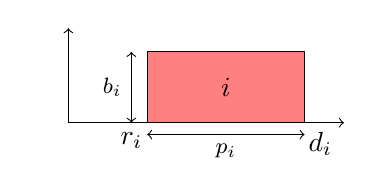
\begin{tikzpicture}
  [yscale=0.3]
  \node[label={[shift={(-0.4,-0.5)}]}] (O) at (0,0) {};
  \draw[fill=red!50] (1,0) rectangle (3,3)   node[midway] {$i$};
  
  \onslide<2-3>{
    \draw[<->] (1,-0.5) -- (3,-0.5) node[midway,below] {\footnotesize $p_i$};
  }
  \onslide<3>{
    \draw[<->] (0.8,0) -- (0.8,3) node[midway,left] {\footnotesize $b_{i}$};
  }
  
  \onslide<4>{
    \draw (0.8,0) node[below] {$r_i$};
    \draw (3.2,0) node[below] {$d_i$};
  }
  
  \draw[->] (O.center) -- (0,4);
  \draw[->] (O.center) -- (3.5,0);


\end{tikzpicture}
